\newif\ifsolutions
\solutionstrue % Show solutions
%\solutionsfalse % Hide solutions

\documentclass{article}
\usepackage{geometry}
\geometry{margin=1in}
\usepackage{tikz}
\usepackage{amssymb}

% fleqn allows setting indent of display math
\usepackage[fleqn]{amsmath}
\setlength{\mathindent}{0pt} % Set indent
% Disable equation numbering (https://tex.stackexchange.com/a/360378)
\makeatletter
\renewcommand\tagform@[1]{}
\makeatother

% Allow Unicode (some, e.g., © and £ at least)
% https://tex.stackexchange.com/questions/370278/is-there-any-reason-to-use-inputenc
\usepackage[utf8]{inputenc}

% Hyperlinks
\usepackage{hyperref}
\hypersetup{colorlinks=true, urlcolor=blue, linkcolor=blue}

% Prevent indentation of paragraphs
\setlength\parindent{0pt}
\setlength{\parskip}{\baselineskip}

% Spacing above/below equations
% https://tex.stackexchange.com/a/69678
\AtBeginDocument{%
 \abovedisplayskip=-\parskip
 \abovedisplayshortskip=-\parskip
 \belowdisplayskip=0pt
 \belowdisplayshortskip=0pt
}

% Allow 3 additional subsection levels
% https://tex.stackexchange.com/a/60212
\usepackage{titlesec}
\setcounter{secnumdepth}{6}
% H4 in HTML
\titleformat{\paragraph}{\normalfont\normalsize\bfseries}{\theparagraph}{1em}{}
\titlespacing*{\paragraph}{0pt}{3.25ex plus 1ex minus .2ex}{1.5ex plus .2ex}
% H5 in HTML
\titleformat{\subparagraph}{\normalfont\normalsize\bfseries}{\thesubparagraph}{1em}{}
\titlespacing*{\subparagraph}{0pt}{3.25ex plus 1ex minus .2ex}{1.5ex plus .2ex}
% H6 in HTML
\titleformat{\subsubparagraph}{\normalfont\normalsize\bfseries}{\thesubsubparagraph}{1em}{}
\titlespacing*{\subsubparagraph}{0pt}{3.25ex plus 1ex minus .2ex}{1.5ex plus .2ex}

% So enumerate at all levels is numbers
% https://tex.stackexchange.com/questions/78842/nested-enumeration-numbering
\renewcommand{\labelenumii}{\arabic{enumii}.}
\renewcommand{\labelenumiii}{\arabic{enumiii}.}
\renewcommand{\labelenumiv}{\arabic{enumiv}.}

\renewcommand{\mbox}{\text}
\newcommand{\ds}[0]{\displaystyle}
\newcommand{\ihat}[0]{\hat{\boldsymbol{\imath}}}
\newcommand{\jhat}[0]{\hat{\boldsymbol{\jmath}}}
\newcommand{\khat}[0]{\hat{\boldsymbol{k}}}
\newcommand{\xhat}[0]{\hat{\mathbf{x}}}
\newcommand{\yhat}[0]{\hat{\mathbf{y}}}
\newcommand{\zhat}[0]{\hat{\mathbf{z}}}
\newcommand{\rhat}[0]{\hat{\mathbf{r}}}
\newcommand{\bfvec}[1]{\vec{\mathbf{#1}}}
\newcommand{\bfcdot}[0]{\boldsymbol{\cdot}}

\usepackage{fancyhdr}
\pagestyle{fancy}
\lhead{Electric Flux}
\rhead{\thepage}
\fancyfoot{}

\begin{document}

\section{Overview}

Several calculations must be performed to use Gauss's law to find the electric field for a system of charges (if possible). First, the electric flux through a closed surface must be found. Second, the amount of charge inside the closed surface must be found. In this activity, you will compute the electric flux through open and closed surfaces.

Electric flux, $\Phi_E$, is the integral of $\bfvec{E}\bfcdot d\bfvec{A}$ over a surface:

$$
\Phi_E=\int\bfvec{E}\bfcdot d\bfvec{A}
$$

When the magnitude and direction of $\bfvec{E}$ is the same at all points on the surface, the integral simplifies to 

$$
\Phi_E = \bfvec{E}\bfcdot \bfvec{A}=\bfvec{E}\bfcdot \hat{\mathbf{n}}A
$$

where $\hat{\mathbf{n}}$ is a unit vector perpendicular to the surface with area $A$. Electric flux is a scalar quantity because it results from the dot product of two vectors (similar to work, which is the dot product of a force vector and displacement vector).

The textbook covers several other forms for $\Phi_E$. The equation $\Phi_E = \bfvec{E}\bfcdot \hat{\mathbf{n}}A$ can also be written as

$$
\Phi_E = E_{\perp}A
$$

where $E_{\perp}$ is the component of $\bfvec{E}$ that is perpendicular to $A$. If the perpendicular component of $\bfvec{E}$ is in the same direction as the normal direction for $\bfvec{A}$, $E_{\perp}$ is positive. If the perpendicular component of $\bfvec{E}$ is in the opposite direction as the normal direction for $\bfvec{A}$, $E_{\perp}$ is negative.

A final form is

$$
\Phi_E = EA\cos\theta
$$

where $\theta$ is the angle between the $\bfvec{E}$ and $\bfvec{A}$ vectors.

Any of these equations can be used, and students are encouraged to use the one they are more comfortable with and ideally understand the relationship between the different equations. When finding $\theta$ is simple based on a diagram, $EA\cos\theta$ is usually the easiest to use. When $\bfvec{E}$ and/or $\hat{\mathbf{n}}$ has three components, $\bfvec{E}\bfcdot \hat{\mathbf{n}}A$ is usually easier to use.

\newpage

\section{$\Phi_E$ Through Open Surface}

\subsection{Problem I}

\begin{enumerate}

  \item a. Draw an area vector $\bfvec{A}=\hat{\mathbf{n}}A$ on the following figure, where $A$ is the area of the dotted rectangle.

        \ifsolutions
        \textbf{Answer}

        

\tikzset{every picture/.style={line width=0.75pt}} %set default line width to 0.75pt        

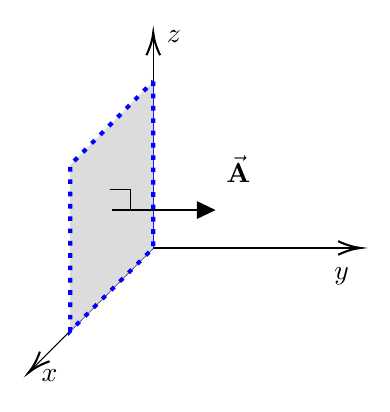
\begin{tikzpicture}[x=0.75pt,y=0.75pt,yscale=-1,xscale=1]
%uncomment if require: \path (0,194); %set diagram left start at 0, and has height of 194

%Straight Lines [id:da24015226796897138] 
\draw    (70,118.27) -- (11.41,176.85) ;
\draw [shift={(10,178.27)}, rotate = 315] [color={rgb, 255:red, 0; green, 0; blue, 0 }  ][line width=0.75]    (10.93,-3.29) .. controls (6.95,-1.4) and (3.31,-0.3) .. (0,0) .. controls (3.31,0.3) and (6.95,1.4) .. (10.93,3.29)   ;
%Straight Lines [id:da043885742210110434] 
\draw    (70,118.27) -- (168,118.27) ;
\draw [shift={(170,118.27)}, rotate = 180] [color={rgb, 255:red, 0; green, 0; blue, 0 }  ][line width=0.75]    (10.93,-3.29) .. controls (6.95,-1.4) and (3.31,-0.3) .. (0,0) .. controls (3.31,0.3) and (6.95,1.4) .. (10.93,3.29)   ;
%Straight Lines [id:da45391014332910573] 
\draw    (70,38.27) -- (70,16.47) ;
\draw [shift={(70,14.47)}, rotate = 90] [color={rgb, 255:red, 0; green, 0; blue, 0 }  ][line width=0.75]    (10.93,-3.29) .. controls (6.95,-1.4) and (3.31,-0.3) .. (0,0) .. controls (3.31,0.3) and (6.95,1.4) .. (10.93,3.29)   ;
%Straight Lines [id:da7578656361659522] 
\draw [color={rgb, 255:red, 0; green, 0; blue, 255 }  ,draw opacity=1 ]   (70,118.27) -- (70,38.27) ;
%Straight Lines [id:da490166639581469] 
\draw [color={rgb, 255:red, 0; green, 0; blue, 255 }  ,draw opacity=1 ] [dash pattern={on 0.84pt off 2.51pt}]  (70,118.27) -- (30,158.27) ;
%Shape: Polygon [id:ds7921940636398519] 
\draw  [color={rgb, 255:red, 0; green, 0; blue, 255 }  ,draw opacity=1 ][fill={rgb, 255:red, 220; green, 220; blue, 220 }  ,fill opacity=1 ][dash pattern={on 1.69pt off 2.76pt}][line width=1.5]  (70,38) -- (70,118.27) -- (30,158.27) -- (30,78.27) -- cycle ;
%Straight Lines [id:da6489051662652563] 
\draw    (50,100) -- (97,100) ;
\draw [shift={(100,100)}, rotate = 180] [fill={rgb, 255:red, 0; green, 0; blue, 0 }  ][line width=0.08]  [draw opacity=0] (8.93,-4.29) -- (0,0) -- (8.93,4.29) -- cycle    ;
%Shape: Right Angle [id:dp8055728240464062] 
\draw   (49,90) -- (59,90) -- (59,100) ;

% Text Node
\draw (15,175.67) node [anchor=north west][inner sep=0.75pt]    {$x$};
% Text Node
\draw (156,126.67) node [anchor=north west][inner sep=0.75pt]    {$y$};
% Text Node
\draw (75.25,12.4) node [anchor=north west][inner sep=0.75pt]    {$z$};
% Text Node
\draw (104,72.4) node [anchor=north west][inner sep=0.75pt]    {$\vec{\mathbf{A}}$};


\end{tikzpicture}

        \else

        

\tikzset{every picture/.style={line width=0.75pt}} %set default line width to 0.75pt        

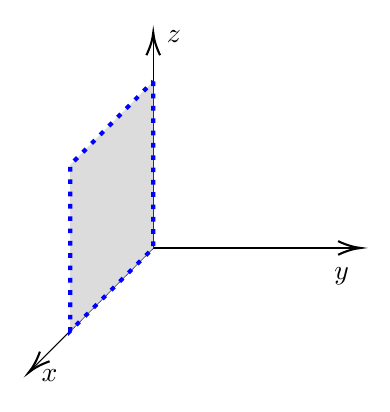
\begin{tikzpicture}[x=0.75pt,y=0.75pt,yscale=-1,xscale=1]
%uncomment if require: \path (0,194); %set diagram left start at 0, and has height of 194

%Straight Lines [id:da6182124976756389] 
\draw    (70,118.27) -- (11.41,176.85) ;
\draw [shift={(10,178.27)}, rotate = 315] [color={rgb, 255:red, 0; green, 0; blue, 0 }  ][line width=0.75]    (10.93,-3.29) .. controls (6.95,-1.4) and (3.31,-0.3) .. (0,0) .. controls (3.31,0.3) and (6.95,1.4) .. (10.93,3.29)   ;
%Straight Lines [id:da054400357518730846] 
\draw    (70,118.27) -- (168,118.27) ;
\draw [shift={(170,118.27)}, rotate = 180] [color={rgb, 255:red, 0; green, 0; blue, 0 }  ][line width=0.75]    (10.93,-3.29) .. controls (6.95,-1.4) and (3.31,-0.3) .. (0,0) .. controls (3.31,0.3) and (6.95,1.4) .. (10.93,3.29)   ;
%Straight Lines [id:da27428028993279274] 
\draw    (70,38.27) -- (70,16.47) ;
\draw [shift={(70,14.47)}, rotate = 90] [color={rgb, 255:red, 0; green, 0; blue, 0 }  ][line width=0.75]    (10.93,-3.29) .. controls (6.95,-1.4) and (3.31,-0.3) .. (0,0) .. controls (3.31,0.3) and (6.95,1.4) .. (10.93,3.29)   ;
%Straight Lines [id:da8528491936420151] 
\draw [color={rgb, 255:red, 0; green, 0; blue, 255 }  ,draw opacity=1 ]   (70,118.27) -- (70,38.27) ;
%Straight Lines [id:da7680185255594141] 
\draw [color={rgb, 255:red, 0; green, 0; blue, 255 }  ,draw opacity=1 ] [dash pattern={on 0.84pt off 2.51pt}]  (70,118.27) -- (30,158.27) ;
%Shape: Polygon [id:ds6468536533951954] 
\draw  [color={rgb, 255:red, 0; green, 0; blue, 255 }  ,draw opacity=1 ][fill={rgb, 255:red, 220; green, 220; blue, 220 }  ,fill opacity=1 ][dash pattern={on 1.69pt off 2.76pt}][line width=1.5]  (70,38) -- (70,118.27) -- (30,158.27) -- (30,78.27) -- cycle ;

% Text Node
\draw (15,175.67) node [anchor=north west][inner sep=0.75pt]    {$x$};
% Text Node
\draw (156,126.67) node [anchor=north west][inner sep=0.75pt]    {$y$};
% Text Node
\draw (75.25,12.4) node [anchor=north west][inner sep=0.75pt]    {$z$};


\end{tikzpicture}

        \fi

        b. Is there only one normal direction to this area? Discuss your reasoning with your group.

        \ifsolutions
        \textbf{Answer}: There are two normal directions, one in $+y$ as shown and another in $-y$ direction. Any surface has two normal vectors. In problems involving a closed surface, the normal direction to use is defined to be the one pointing outwards from the volume the surface encloses. In problems involving an open surface such as this one, you may use either normal direction if the one to use is not specified.
        \else
        \vskip 72pt
        \fi

  \item In this part, use the normal vector for the area in the $y$--direction. For each of the following $\bfvec{E}$ vectors a.-d., draw $\bfvec{E}$ and $\hat{\mathbf{n}}$ on the following diagram, which shows the area in the previous figure when viewed from a point on the positive $z$--axis that is far from the origin. Then, find $\theta$ and compute $\Phi_E$ in terms of the constants $E_o$ and $A$.

        \ifsolutions
        \textbf{Answer}

        \input{figures/Electric_Flux_xz_Plane_Solution_b.tikz}

        a. $\quad\ds\bfvec{E}=E_o\ihat\qquad\phantom{+\frac{E_o}{\sqrt{2}}\jhat}\theta=90^\circ\qquad\qquad\Phi_E=E_oA\cos 90^\circ = 0$

        b. $\quad\ds\bfvec{E}=E_o\jhat\qquad\phantom{+ \frac{E_o}{\sqrt{2}}\jhat}\theta=0^\circ\qquad\qquad\Phi_E=E_oA\cos 0^\circ=E_oA$ 

        c. $\quad\ds\bfvec{E}=E_o\khat\qquad\phantom{+\frac{E_o}{\sqrt{2}}\jhat}\theta=90^\circ\qquad\qquad\Phi_E=E_oA\cos 90^\circ=0$ 

        d. $\quad\ds\bfvec{E}=\frac{E_o}{\sqrt{2}}\ihat + \frac{E_o}{\sqrt{2}}\jhat\qquad\theta=45^\circ\qquad\qquad\Phi_E=E_o A\cos 45^\circ=E_oA/\sqrt{2}$

        Note that $\Phi_E=EA\cos\theta$ and so in d. we need the magnitude $E = |\bfvec{E}| = \sqrt{(E_o/\sqrt{2})^2+(E_o/\sqrt{2})^2)}=E_o$.
        \else

        \input{figures/Electric_Flux_xz_Plane_Sketch.tikz}

        a. $\quad\ds\bfvec{E}=E_o\ihat\qquad\phantom{+\frac{E_o}{\sqrt{2}}\jhat}\theta=\qquad\qquad\Phi_E=$

        b. $\quad\ds\bfvec{E}=E_o\jhat\qquad\phantom{+ \frac{E_o}{\sqrt{2}}\jhat}\theta=\qquad\qquad\Phi_E=$ 

        c. $\quad\ds\bfvec{E}=E_o\khat\qquad\phantom{+\frac{E_o}{\sqrt{2}}\jhat}\theta=\qquad\qquad\Phi_E=$ 

        d. $\quad\ds\bfvec{E}=\frac{E_o}{\sqrt{2}}\ihat + \frac{E_o}{\sqrt{2}}\jhat\qquad\theta=\qquad\qquad\Phi_E=$

        \newpage
        \fi

\end{enumerate}

\subsection{Problem II}

\ifsolutions

\else



\tikzset{every picture/.style={line width=0.75pt}} %set default line width to 0.75pt        

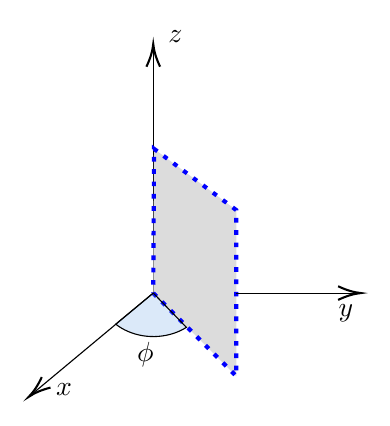
\begin{tikzpicture}[x=0.75pt,y=0.75pt,yscale=-1,xscale=1]
%uncomment if require: \path (0,193); %set diagram left start at 0, and has height of 193

%Straight Lines [id:da25158216828132907] 
\draw    (70,12) -- (70,130) ;
\draw [shift={(70,10)}, rotate = 90] [color={rgb, 255:red, 0; green, 0; blue, 0 }  ][line width=0.75]    (10.93,-3.29) .. controls (6.95,-1.4) and (3.31,-0.3) .. (0,0) .. controls (3.31,0.3) and (6.95,1.4) .. (10.93,3.29)   ;
%Shape: Polygon [id:ds8423391814956749] 
\draw  [color={rgb, 255:red, 0; green, 0; blue, 255 }  ,draw opacity=1 ][fill={rgb, 255:red, 220; green, 220; blue, 220 }  ,fill opacity=1 ][dash pattern={on 1.69pt off 2.76pt}][line width=1.5]  (70,130) -- (110,170) -- (110,90) -- (70.38,60.5) -- cycle ;
%Straight Lines [id:da2527948429112177] 
\draw    (70,130) -- (11.54,178.72) ;
\draw [shift={(10,180)}, rotate = 320.19] [color={rgb, 255:red, 0; green, 0; blue, 0 }  ][line width=0.75]    (10.93,-3.29) .. controls (6.95,-1.4) and (3.31,-0.3) .. (0,0) .. controls (3.31,0.3) and (6.95,1.4) .. (10.93,3.29)   ;
%Straight Lines [id:da06711060098815369] 
\draw    (110,130) -- (168,130) ;
\draw [shift={(170,130)}, rotate = 180] [color={rgb, 255:red, 0; green, 0; blue, 0 }  ][line width=0.75]    (10.93,-3.29) .. controls (6.95,-1.4) and (3.31,-0.3) .. (0,0) .. controls (3.31,0.3) and (6.95,1.4) .. (10.93,3.29)   ;
%Shape: Pie [id:dp17804997975604353] 
\draw  [fill={rgb, 255:red, 74; green, 144; blue, 226 }  ,fill opacity=0.2 ] (85.99,146.51) .. controls (78.16,151.47) and (67.14,152.52) .. (57.8,148.46) .. controls (55.59,147.51) and (53.63,146.33) .. (51.92,144.98) -- (70,130) -- cycle ;

% Text Node
\draw (22,172.4) node [anchor=north west][inner sep=0.75pt]    {$x$};
% Text Node
\draw (158,134.4) node [anchor=north west][inner sep=0.75pt]    {$y$};
% Text Node
\draw (76,2.4) node [anchor=north west][inner sep=0.75pt]    {$z$};
% Text Node
\draw (61,152.4) node [anchor=north west][inner sep=0.75pt]    {$\phi $};


\end{tikzpicture}

\fi

If the area from the previous problem is rotated by $\phi=45^\circ$ around the $z$--axis, draw the area as it would look from a point on the positive $z$-axis that is far from the origin (that is, draw the projection onto the $x$--$y$ plane). Then draw $\hat{\mathbf{n}}$ and $\bfvec{E}$ for each of the electric fields a.--d.

\ifsolutions
\textbf{Solution} 

Note that the symbol $\odot$ in c. indicates a vector pointing out of the page.



\tikzset{every picture/.style={line width=0.75pt}} %set default line width to 0.75pt        

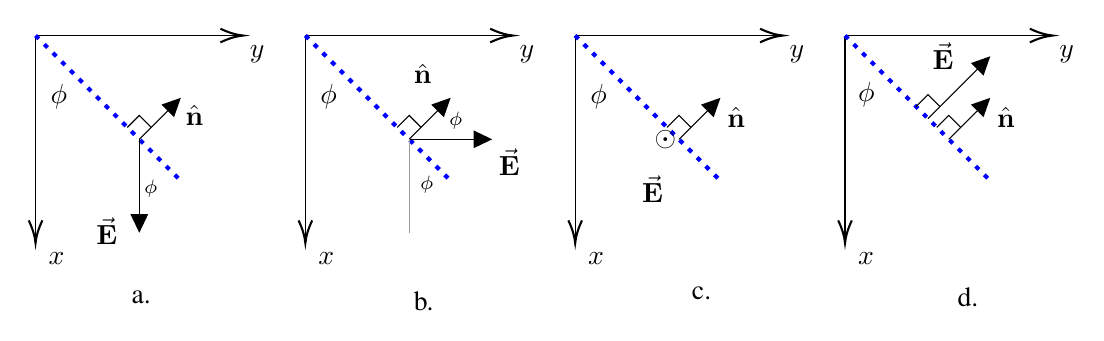
\begin{tikzpicture}[x=0.75pt,y=0.75pt,yscale=-1,xscale=1]
%uncomment if require: \path (0,171); %set diagram left start at 0, and has height of 171

%Straight Lines [id:da702573714141205] 
\draw    (10,20) -- (10,118) ;
\draw [shift={(10,120)}, rotate = 270] [color={rgb, 255:red, 0; green, 0; blue, 0 }  ][line width=0.75]    (10.93,-3.29) .. controls (6.95,-1.4) and (3.31,-0.3) .. (0,0) .. controls (3.31,0.3) and (6.95,1.4) .. (10.93,3.29)   ;
%Straight Lines [id:da43004021154585925] 
\draw    (10,20) -- (108,20) ;
\draw [shift={(110,20)}, rotate = 180] [color={rgb, 255:red, 0; green, 0; blue, 0 }  ][line width=0.75]    (10.93,-3.29) .. controls (6.95,-1.4) and (3.31,-0.3) .. (0,0) .. controls (3.31,0.3) and (6.95,1.4) .. (10.93,3.29)   ;
%Straight Lines [id:da8907866746998676] 
\draw    (140,20) -- (238,20) ;
\draw [shift={(240,20)}, rotate = 180] [color={rgb, 255:red, 0; green, 0; blue, 0 }  ][line width=0.75]    (10.93,-3.29) .. controls (6.95,-1.4) and (3.31,-0.3) .. (0,0) .. controls (3.31,0.3) and (6.95,1.4) .. (10.93,3.29)   ;
%Straight Lines [id:da6087551199791568] 
\draw    (270,20) -- (368,20) ;
\draw [shift={(370,20)}, rotate = 180] [color={rgb, 255:red, 0; green, 0; blue, 0 }  ][line width=0.75]    (10.93,-3.29) .. controls (6.95,-1.4) and (3.31,-0.3) .. (0,0) .. controls (3.31,0.3) and (6.95,1.4) .. (10.93,3.29)   ;
%Straight Lines [id:da24396661001332443] 
\draw    (400,20) -- (498,20) ;
\draw [shift={(500,20)}, rotate = 180] [color={rgb, 255:red, 0; green, 0; blue, 0 }  ][line width=0.75]    (10.93,-3.29) .. controls (6.95,-1.4) and (3.31,-0.3) .. (0,0) .. controls (3.31,0.3) and (6.95,1.4) .. (10.93,3.29)   ;
%Straight Lines [id:da24695355939175045] 
\draw    (140,20) -- (140,118) ;
\draw [shift={(140,120)}, rotate = 270] [color={rgb, 255:red, 0; green, 0; blue, 0 }  ][line width=0.75]    (10.93,-3.29) .. controls (6.95,-1.4) and (3.31,-0.3) .. (0,0) .. controls (3.31,0.3) and (6.95,1.4) .. (10.93,3.29)   ;
%Straight Lines [id:da8005467419213836] 
\draw    (270,20) -- (270,118) ;
\draw [shift={(270,120)}, rotate = 270] [color={rgb, 255:red, 0; green, 0; blue, 0 }  ][line width=0.75]    (10.93,-3.29) .. controls (6.95,-1.4) and (3.31,-0.3) .. (0,0) .. controls (3.31,0.3) and (6.95,1.4) .. (10.93,3.29)   ;
%Straight Lines [id:da5901656620510045] 
\draw    (400,20) -- (400,118) ;
\draw [shift={(400,120)}, rotate = 270] [color={rgb, 255:red, 0; green, 0; blue, 0 }  ][line width=0.75]    (10.93,-3.29) .. controls (6.95,-1.4) and (3.31,-0.3) .. (0,0) .. controls (3.31,0.3) and (6.95,1.4) .. (10.93,3.29)   ;
%Straight Lines [id:da7113561546411471] 
\draw [color={rgb, 255:red, 0; green, 0; blue, 255 }  ,draw opacity=1 ][line width=1.5]  [dash pattern={on 1.69pt off 2.76pt}]  (10,20) -- (80,90) ;
%Straight Lines [id:da4137691598782649] 
\draw    (60,70) -- (77.88,52.12) ;
\draw [shift={(80,50)}, rotate = 135] [fill={rgb, 255:red, 0; green, 0; blue, 0 }  ][line width=0.08]  [draw opacity=0] (8.93,-4.29) -- (0,0) -- (8.93,4.29) -- cycle    ;
%Straight Lines [id:da6743497193490973] 
\draw [color={rgb, 255:red, 0; green, 0; blue, 255 }  ,draw opacity=1 ][line width=1.5]  [dash pattern={on 1.69pt off 2.76pt}]  (140,20) -- (210,90) ;
%Straight Lines [id:da5189204521474442] 
\draw    (190,70) -- (207.88,52.12) ;
\draw [shift={(210,50)}, rotate = 135] [fill={rgb, 255:red, 0; green, 0; blue, 0 }  ][line width=0.08]  [draw opacity=0] (8.93,-4.29) -- (0,0) -- (8.93,4.29) -- cycle    ;
%Straight Lines [id:da29791216748386296] 
\draw [color={rgb, 255:red, 0; green, 0; blue, 255 }  ,draw opacity=1 ][line width=1.5]  [dash pattern={on 1.69pt off 2.76pt}]  (270,20) -- (340,90) ;
%Straight Lines [id:da3970999332308571] 
\draw [color={rgb, 255:red, 0; green, 0; blue, 255 }  ,draw opacity=1 ][line width=1.5]  [dash pattern={on 1.69pt off 2.76pt}]  (400,20) -- (470,90) ;
%Straight Lines [id:da7830834247062961] 
\draw    (450,70) -- (467.88,52.12) ;
\draw [shift={(470,50)}, rotate = 135] [fill={rgb, 255:red, 0; green, 0; blue, 0 }  ][line width=0.08]  [draw opacity=0] (8.93,-4.29) -- (0,0) -- (8.93,4.29) -- cycle    ;
%Straight Lines [id:da3780191899677152] 
\draw    (60,70) -- (60,112) ;
\draw [shift={(60,115)}, rotate = 270] [fill={rgb, 255:red, 0; green, 0; blue, 0 }  ][line width=0.08]  [draw opacity=0] (8.93,-4.29) -- (0,0) -- (8.93,4.29) -- cycle    ;
%Straight Lines [id:da19436962599794438] 
\draw    (190,70) -- (227,70) ;
\draw [shift={(230,70)}, rotate = 180] [fill={rgb, 255:red, 0; green, 0; blue, 0 }  ][line width=0.08]  [draw opacity=0] (8.93,-4.29) -- (0,0) -- (8.93,4.29) -- cycle    ;
%Straight Lines [id:da5125722671804134] 
\draw    (440,60) -- (467.88,32.12) ;
\draw [shift={(470,30)}, rotate = 135] [fill={rgb, 255:red, 0; green, 0; blue, 0 }  ][line width=0.08]  [draw opacity=0] (8.93,-4.29) -- (0,0) -- (8.93,4.29) -- cycle    ;
%Straight Lines [id:da4201122342964998] 
\draw    (320,70) -- (337.88,52.12) ;
\draw [shift={(340,50)}, rotate = 135] [fill={rgb, 255:red, 0; green, 0; blue, 0 }  ][line width=0.08]  [draw opacity=0] (8.93,-4.29) -- (0,0) -- (8.93,4.29) -- cycle    ;
%Straight Lines [id:da5850513565784372] 
\draw [color={rgb, 255:red, 155; green, 155; blue, 155 }  ,draw opacity=1 ]   (190,70) -- (190,115) ;
%Shape: Right Angle [id:dp3080397474447747] 
\draw   (65.76,64.24) -- (60,58.48) -- (54.24,64.24) ;
%Shape: Right Angle [id:dp8812037978944036] 
\draw   (195.76,64.24) -- (190,58.48) -- (184.24,64.24) ;
%Shape: Right Angle [id:dp2394903386053333] 
\draw   (325.76,64.24) -- (320,58.48) -- (314.24,64.24) ;
%Shape: Right Angle [id:dp17721568864317883] 
\draw   (455.76,64.24) -- (450,58.48) -- (444.24,64.24) ;
%Shape: Right Angle [id:dp29393462612364685] 
\draw   (445.76,54.24) -- (440,48.48) -- (434.24,54.24) ;

% Text Node
\draw (15,123.4) node [anchor=north west][inner sep=0.75pt]    {$x$};
% Text Node
\draw (112,23.4) node [anchor=north west][inner sep=0.75pt]    {$y$};
% Text Node
\draw (145,123.4) node [anchor=north west][inner sep=0.75pt]    {$x$};
% Text Node
\draw (242,23.4) node [anchor=north west][inner sep=0.75pt]    {$y$};
% Text Node
\draw (275,123.4) node [anchor=north west][inner sep=0.75pt]    {$x$};
% Text Node
\draw (372,23.4) node [anchor=north west][inner sep=0.75pt]    {$y$};
% Text Node
\draw (405,123.4) node [anchor=north west][inner sep=0.75pt]    {$x$};
% Text Node
\draw (502,23.4) node [anchor=north west][inner sep=0.75pt]    {$y$};
% Text Node
\draw (55,142) node [anchor=north west][inner sep=0.75pt]   [align=left] {{\fontfamily{ptm}\selectfont a.}};
% Text Node
\draw (191,142) node [anchor=north west][inner sep=0.75pt]   [align=left] {{\fontfamily{ptm}\selectfont b.}};
% Text Node
\draw (325,140) node [anchor=north west][inner sep=0.75pt]   [align=left] {{\fontfamily{ptm}\selectfont c.}};
% Text Node
\draw (453,140) node [anchor=north west][inner sep=0.75pt]   [align=left] {{\fontfamily{ptm}\selectfont d.}};
% Text Node
\draw (81,52.4) node [anchor=north west][inner sep=0.75pt]    {$\hat{\mathbf{n}}$};
% Text Node
\draw (191,32.4) node [anchor=north west][inner sep=0.75pt]    {$\hat{\mathbf{n}}$};
% Text Node
\draw (342,53.4) node [anchor=north west][inner sep=0.75pt]    {$\hat{\mathbf{n}}$};
% Text Node
\draw (472,53.4) node [anchor=north west][inner sep=0.75pt]    {$\hat{\mathbf{n}}$};
% Text Node
\draw (38,106.4) node [anchor=north west][inner sep=0.75pt]    {$\vec{\mathbf{E}}$};
% Text Node
\draw (232,73.4) node [anchor=north west][inner sep=0.75pt]    {$\vec{\mathbf{E}}$};
% Text Node
\draw (307,64.4) node [anchor=north west][inner sep=0.75pt]    {$\odot $};
% Text Node
\draw (301,86.4) node [anchor=north west][inner sep=0.75pt]    {$\vec{\mathbf{E}}$};
% Text Node
\draw (441,22.4) node [anchor=north west][inner sep=0.75pt]    {$\vec{\mathbf{E}}$};
% Text Node
\draw (16,42.4) node [anchor=north west][inner sep=0.75pt]    {$\phi $};
% Text Node
\draw (61,88.4) node [anchor=north west][inner sep=0.75pt]  [font=\scriptsize]  {$\phi $};
% Text Node
\draw (208,55.4) node [anchor=north west][inner sep=0.75pt]  [font=\scriptsize]  {$\phi $};
% Text Node
\draw (146,42.4) node [anchor=north west][inner sep=0.75pt]    {$\phi $};
% Text Node
\draw (276,42.4) node [anchor=north west][inner sep=0.75pt]    {$\phi $};
% Text Node
\draw (405,41.4) node [anchor=north west][inner sep=0.75pt]    {$\phi $};
% Text Node
\draw (194,86.4) node [anchor=north west][inner sep=0.75pt]  [font=\scriptsize]  {$\phi $};


\end{tikzpicture}


a. $\quad\ds\bfvec{E}=E_o\ihat\quad\theta=\phi+90^\circ=135^\circ\quad\Phi_E=E_oA\cos 135^\circ=-E_oA\cos 45^\circ=-E_oA/\sqrt{2}$

b. $\quad\ds\bfvec{E}=E_o\jhat\quad\theta=\phi=45^\circ\quad\Phi_E=E_oA\cos 45^\circ=E_oA/\sqrt{2}$ 

c. $\quad\ds\bfvec{E}=E_o\khat\quad\theta=90^\circ\quad\Phi_E=E_oA\cos 90^\circ=0$ 

d. $\quad\ds\bfvec{E}=\frac{E_o}{\sqrt{2}}\ihat + \frac{E_o}{\sqrt{2}}\jhat\quad\theta=90^\circ\quad\Phi_E=E_oA\cos 90^\circ=0$
\else



\tikzset{every picture/.style={line width=0.75pt}} %set default line width to 0.75pt        

\begin{tikzpicture}[x=0.75pt,y=0.75pt,yscale=-1,xscale=1]
%uncomment if require: \path (0,171); %set diagram left start at 0, and has height of 171

%Straight Lines [id:da40892576218271226] 
\draw [color={rgb, 255:red, 0; green, 0; blue, 0 }  ,draw opacity=1 ][line width=0.75]    (13,100) -- (13,20) ;
%Straight Lines [id:da5033158460564655] 
\draw    (13,90) -- (13,118) ;
\draw [shift={(13,120)}, rotate = 270] [color={rgb, 255:red, 0; green, 0; blue, 0 }  ][line width=0.75]    (10.93,-3.29) .. controls (6.95,-1.4) and (3.31,-0.3) .. (0,0) .. controls (3.31,0.3) and (6.95,1.4) .. (10.93,3.29)   ;
%Straight Lines [id:da02776586237775347] 
\draw    (13,20) -- (111,20) ;
\draw [shift={(113,20)}, rotate = 180] [color={rgb, 255:red, 0; green, 0; blue, 0 }  ][line width=0.75]    (10.93,-3.29) .. controls (6.95,-1.4) and (3.31,-0.3) .. (0,0) .. controls (3.31,0.3) and (6.95,1.4) .. (10.93,3.29)   ;
%Straight Lines [id:da4939234227411431] 
\draw    (143,90) -- (143,118) ;
\draw [shift={(143,120)}, rotate = 270] [color={rgb, 255:red, 0; green, 0; blue, 0 }  ][line width=0.75]    (10.93,-3.29) .. controls (6.95,-1.4) and (3.31,-0.3) .. (0,0) .. controls (3.31,0.3) and (6.95,1.4) .. (10.93,3.29)   ;
%Straight Lines [id:da04453092163787442] 
\draw    (143,20) -- (241,20) ;
\draw [shift={(243,20)}, rotate = 180] [color={rgb, 255:red, 0; green, 0; blue, 0 }  ][line width=0.75]    (10.93,-3.29) .. controls (6.95,-1.4) and (3.31,-0.3) .. (0,0) .. controls (3.31,0.3) and (6.95,1.4) .. (10.93,3.29)   ;
%Straight Lines [id:da9811994499622934] 
\draw    (273,90) -- (273,118) ;
\draw [shift={(273,120)}, rotate = 270] [color={rgb, 255:red, 0; green, 0; blue, 0 }  ][line width=0.75]    (10.93,-3.29) .. controls (6.95,-1.4) and (3.31,-0.3) .. (0,0) .. controls (3.31,0.3) and (6.95,1.4) .. (10.93,3.29)   ;
%Straight Lines [id:da0467407683586889] 
\draw    (273,20) -- (371,20) ;
\draw [shift={(373,20)}, rotate = 180] [color={rgb, 255:red, 0; green, 0; blue, 0 }  ][line width=0.75]    (10.93,-3.29) .. controls (6.95,-1.4) and (3.31,-0.3) .. (0,0) .. controls (3.31,0.3) and (6.95,1.4) .. (10.93,3.29)   ;
%Straight Lines [id:da44721013430709533] 
\draw    (403,90) -- (403,118) ;
\draw [shift={(403,120)}, rotate = 270] [color={rgb, 255:red, 0; green, 0; blue, 0 }  ][line width=0.75]    (10.93,-3.29) .. controls (6.95,-1.4) and (3.31,-0.3) .. (0,0) .. controls (3.31,0.3) and (6.95,1.4) .. (10.93,3.29)   ;
%Straight Lines [id:da08970539993195059] 
\draw    (403,20) -- (501,20) ;
\draw [shift={(503,20)}, rotate = 180] [color={rgb, 255:red, 0; green, 0; blue, 0 }  ][line width=0.75]    (10.93,-3.29) .. controls (6.95,-1.4) and (3.31,-0.3) .. (0,0) .. controls (3.31,0.3) and (6.95,1.4) .. (10.93,3.29)   ;
%Straight Lines [id:da5925972402309474] 
\draw [color={rgb, 255:red, 0; green, 0; blue, 0 }  ,draw opacity=1 ][line width=0.75]    (143,100) -- (143,20) ;
%Straight Lines [id:da6481009892507923] 
\draw [color={rgb, 255:red, 0; green, 0; blue, 0 }  ,draw opacity=1 ][line width=0.75]    (273,100) -- (273,20) ;
%Straight Lines [id:da5821047608502132] 
\draw [color={rgb, 255:red, 0; green, 0; blue, 0 }  ,draw opacity=1 ][line width=0.75]    (403,100) -- (403,20) ;

% Text Node
\draw (15,123.4) node [anchor=north west][inner sep=0.75pt]    {$x$};
% Text Node
\draw (101,27.4) node [anchor=north west][inner sep=0.75pt]    {$y$};
% Text Node
\draw (145,123.4) node [anchor=north west][inner sep=0.75pt]    {$x$};
% Text Node
\draw (231,26.4) node [anchor=north west][inner sep=0.75pt]    {$y$};
% Text Node
\draw (275,123.4) node [anchor=north west][inner sep=0.75pt]    {$x$};
% Text Node
\draw (361,26.4) node [anchor=north west][inner sep=0.75pt]    {$y$};
% Text Node
\draw (405,123.4) node [anchor=north west][inner sep=0.75pt]    {$x$};
% Text Node
\draw (491,26.4) node [anchor=north west][inner sep=0.75pt]    {$y$};
% Text Node
\draw (55,142) node [anchor=north west][inner sep=0.75pt]   [align=left] {{\fontfamily{ptm}\selectfont a.}};
% Text Node
\draw (191,142) node [anchor=north west][inner sep=0.75pt]   [align=left] {{\fontfamily{ptm}\selectfont b.}};
% Text Node
\draw (325,140) node [anchor=north west][inner sep=0.75pt]   [align=left] {{\fontfamily{ptm}\selectfont c.}};
% Text Node
\draw (453,140) node [anchor=north west][inner sep=0.75pt]   [align=left] {{\fontfamily{ptm}\selectfont d.}};


\end{tikzpicture}


a. $\quad\ds\bfvec{E}=E_o\ihat\qquad\phantom{+\frac{E_o}{\sqrt{2}}\jhat}\theta=\qquad\qquad\Phi_E=$

b. $\quad\ds\bfvec{E}=E_o\jhat\qquad\phantom{+ \frac{E_o}{\sqrt{2}}\jhat}\theta=\qquad\qquad\Phi_E=$ 

c. $\quad\ds\bfvec{E}=E_o\khat\qquad\phantom{+\frac{E_o}{\sqrt{2}}\jhat}\theta=\qquad\qquad\Phi_E=$ 

d. $\quad\ds\bfvec{E}=\frac{E_o}{\sqrt{2}}\ihat + \frac{E_o}{\sqrt{2}}\jhat\qquad\theta=\qquad\qquad\Phi_E=$
\fi

\section{$\Phi_E$ Through Closed Surface}

In the previous problem, you computed the flux through an open surface. You should have noted that there are two area vectors to an open surface -- imagine your hand being an open surface. You can put the pencil (1) on the top of your hand with the tip pointing up or (2) in your palm with the tip pointing down. The pencil represents the vector, and the tip indicates the direction.

Gauss's law, which involves electric flux, always involves a closed surface (if you put water inside a closed surface, it will not leak out). For Gauss's law, there is a convention for which area vector to choose -- it is the one that points outwards from the volume that the surface encloses. 

In the following example, the electric flux is computed through a closed surface (the sides of a cube) by finding the flux through each of the sides of the cube. The total electric flux is the sum of the fluxes through each side.

%The reason we are interested in knowing the flux through a closed surface is due to a remarkable mathematical result known as Gauss's law. Suppose that you can measure the electric field on an arbitrary and closed surface. The net electric flux through the surface that you compute is related to the total amount of charge inside the surface! For example, if you are given the electric field at all points on the surface of a closed cardboard box, you can compute the total charge inside the box without having to open it. 

With Coulomb's law, we are given the location and values of charges, and we compute the electric field anywhere in space. With Gauss's law, we can do the reverse -- given an electric field on the surface of a small volume of space, we can compute the charge in the volume. (If the volume is large, we can only compute the amount of charge enclosed in the volume; however, if the closed surface volume approaches zero, we can compute the amount of charge at a point in space.)

\subsection{Example}



\tikzset{every picture/.style={line width=0.75pt}} %set default line width to 0.75pt        

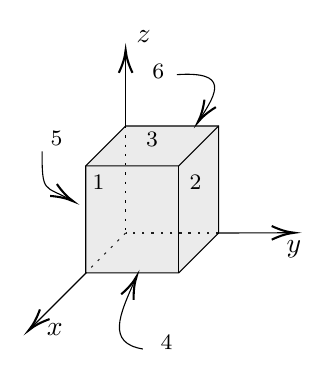
\begin{tikzpicture}[x=0.75pt,y=0.75pt,yscale=-1,xscale=1]
%uncomment if require: \path (0,177); %set diagram left start at 0, and has height of 177

%Straight Lines [id:da6367799622029096] 
\draw  [dash pattern={on 0.84pt off 2.51pt}]  (71.2,110.8) -- (52,130) ;
%Straight Lines [id:da6001535337839026] 
\draw  [dash pattern={on 0.84pt off 2.51pt}]  (116,110.8) -- (71.2,110.8) ;
%Shape: Cube [id:dp04342558315379508] 
\draw  [fill={rgb, 255:red, 155; green, 155; blue, 155 }  ,fill opacity=0.2 ] (52,78.45) -- (71.2,59.25) -- (116,59.25) -- (116,110.8) -- (96.8,130) -- (52,130) -- cycle ; \draw   (116,59.25) -- (96.8,78.45) -- (52,78.45) ; \draw   (96.8,78.45) -- (96.8,130) ;
%Straight Lines [id:da33768233880307563] 
\draw  [dash pattern={on 0.84pt off 2.51pt}]  (71.2,59.25) -- (71.2,110.8) ;
%Straight Lines [id:da8556566864205468] 
\draw    (52.17,130) -- (25.91,156.25) ;
\draw [shift={(24.5,157.67)}, rotate = 315] [color={rgb, 255:red, 0; green, 0; blue, 0 }  ][line width=0.75]    (10.93,-3.29) .. controls (6.95,-1.4) and (3.31,-0.3) .. (0,0) .. controls (3.31,0.3) and (6.95,1.4) .. (10.93,3.29)   ;
%Straight Lines [id:da7859931310096506] 
\draw    (116,110.8) -- (150.5,110.67) ;
\draw [shift={(152.5,110.67)}, rotate = 179.79] [color={rgb, 255:red, 0; green, 0; blue, 0 }  ][line width=0.75]    (10.93,-3.29) .. controls (6.95,-1.4) and (3.31,-0.3) .. (0,0) .. controls (3.31,0.3) and (6.95,1.4) .. (10.93,3.29)   ;
%Straight Lines [id:da7670470282458908] 
\draw    (71.2,59.25) -- (71.2,24.67) ;
\draw [shift={(71.2,22.67)}, rotate = 90] [color={rgb, 255:red, 0; green, 0; blue, 0 }  ][line width=0.75]    (10.93,-3.29) .. controls (6.95,-1.4) and (3.31,-0.3) .. (0,0) .. controls (3.31,0.3) and (6.95,1.4) .. (10.93,3.29)   ;
%Curve Lines [id:da43558820809067944] 
\draw    (79.5,166.67) .. controls (62.04,163.76) and (68.1,150.5) .. (75.78,133.28) ;
\draw [shift={(76.5,131.67)}, rotate = 113.96] [color={rgb, 255:red, 0; green, 0; blue, 0 }  ][line width=0.75]    (10.93,-3.29) .. controls (6.95,-1.4) and (3.31,-0.3) .. (0,0) .. controls (3.31,0.3) and (6.95,1.4) .. (10.93,3.29)   ;
%Curve Lines [id:da8847199212806154] 
\draw    (30.93,71.49) .. controls (30.93,91.65) and (31.85,87.85) .. (44.31,94.59) ;
\draw [shift={(45.93,95.49)}, rotate = 209.74] [color={rgb, 255:red, 0; green, 0; blue, 0 }  ][line width=0.75]    (10.93,-3.29) .. controls (6.95,-1.4) and (3.31,-0.3) .. (0,0) .. controls (3.31,0.3) and (6.95,1.4) .. (10.93,3.29)   ;
%Curve Lines [id:da0524228217917051] 
\draw    (95.93,34.49) .. controls (120.89,32.85) and (115.44,42.92) .. (107,55.86) ;
\draw [shift={(105.93,57.49)}, rotate = 303.27] [color={rgb, 255:red, 0; green, 0; blue, 0 }  ][line width=0.75]    (10.93,-3.29) .. controls (6.95,-1.4) and (3.31,-0.3) .. (0,0) .. controls (3.31,0.3) and (6.95,1.4) .. (10.93,3.29)   ;

% Text Node
\draw (54,81.85) node [anchor=north west][inner sep=0.75pt]  [font=\footnotesize]  {$1$};
% Text Node
\draw (100.8,81.85) node [anchor=north west][inner sep=0.75pt]  [font=\footnotesize]  {$2$};
% Text Node
\draw (79.87,60.77) node [anchor=north west][inner sep=0.75pt]  [font=\footnotesize,rotate=-0.7]  {$3$};
% Text Node
\draw (32,153.4) node [anchor=north west][inner sep=0.75pt]    {$x$};
% Text Node
\draw (147.5,113.07) node [anchor=north west][inner sep=0.75pt]    {$y$};
% Text Node
\draw (86.87,158.77) node [anchor=north west][inner sep=0.75pt]  [font=\footnotesize,rotate=-0.7]  {$4$};
% Text Node
\draw (33.87,60.42) node [anchor=north west][inner sep=0.75pt]  [font=\footnotesize,rotate=-0.7]  {$5$};
% Text Node
\draw (75.25,12.13) node [anchor=north west][inner sep=0.75pt]    {$z$};
% Text Node
\draw (82.87,28.42) node [anchor=north west][inner sep=0.75pt]  [font=\footnotesize,rotate=-0.7]  {$6$};


\end{tikzpicture}


Find the flux through the six labeled faces of the cube with side area $A$ when the electric field is everywhere in the $+z$ direction with magnitude $E_o$.

{\bf Answer} This example is similar to Example 22.2a pg 728 in the textbook. The electric field is parallel to surfaces 1, 2, 5, and 6. For each of these surfaces, $\theta=90^\circ$, and $\cos( 90^\circ)=0$. 

%We'll solve it using two methods. The first method is useful when the electric field is either parallel or perpendicular to all surfaces. The second method is useful for more general cases, such as problem 3.3.

%Method I

$\Phi_E^{1}=\Phi_E^{2}=\Phi_E^{5}=\Phi_E^{6}=0$

By convention, the normal direction for surface 3 is outwards from the volume, which is in the $+z$-direction. The electric field is in the same direction, so $\theta=0$ and

$\Phi_E^{3}=E_oA\cos0^\circ=E_oA$

The normal direction for the bottom surface is downwards, which is in the opposite direction as the electric field, so $\theta=180^\circ$ and

$\Phi_E^{4}=E_oA\cos 180^\circ=-E_oA$

The total flux through the cube, $\Phi_E^1+...+\Phi_E^6$, is zero. Using the analogy of electric field lines representing flow lines, every electric field line that enters the cube exits, so the flow in equals the flow out. (Perhaps confusingly, by convention, flow out of a volume corresponds to a positive flux. This convention for electric flux is used because in Gauss's law, a net flux out of a closed surface corresponds to a net positive charge inside the surface.)

The motivation for computing electric flux through a closed surface is that it appears in Gauss's law, which is covered in a later activity. Based on Gauss's law, we can conclude that the net charge in the cube is zero because the net flux through the cube's surface is zero.

\ifsolutions

\else

\newpage
\fi

\subsection{Problem}



\tikzset{every picture/.style={line width=0.75pt}} %set default line width to 0.75pt        

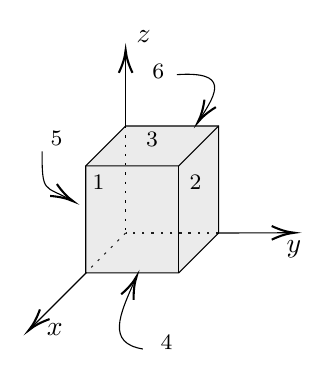
\begin{tikzpicture}[x=0.75pt,y=0.75pt,yscale=-1,xscale=1]
%uncomment if require: \path (0,177); %set diagram left start at 0, and has height of 177

%Straight Lines [id:da6367799622029096] 
\draw  [dash pattern={on 0.84pt off 2.51pt}]  (71.2,110.8) -- (52,130) ;
%Straight Lines [id:da6001535337839026] 
\draw  [dash pattern={on 0.84pt off 2.51pt}]  (116,110.8) -- (71.2,110.8) ;
%Shape: Cube [id:dp04342558315379508] 
\draw  [fill={rgb, 255:red, 155; green, 155; blue, 155 }  ,fill opacity=0.2 ] (52,78.45) -- (71.2,59.25) -- (116,59.25) -- (116,110.8) -- (96.8,130) -- (52,130) -- cycle ; \draw   (116,59.25) -- (96.8,78.45) -- (52,78.45) ; \draw   (96.8,78.45) -- (96.8,130) ;
%Straight Lines [id:da33768233880307563] 
\draw  [dash pattern={on 0.84pt off 2.51pt}]  (71.2,59.25) -- (71.2,110.8) ;
%Straight Lines [id:da8556566864205468] 
\draw    (52.17,130) -- (25.91,156.25) ;
\draw [shift={(24.5,157.67)}, rotate = 315] [color={rgb, 255:red, 0; green, 0; blue, 0 }  ][line width=0.75]    (10.93,-3.29) .. controls (6.95,-1.4) and (3.31,-0.3) .. (0,0) .. controls (3.31,0.3) and (6.95,1.4) .. (10.93,3.29)   ;
%Straight Lines [id:da7859931310096506] 
\draw    (116,110.8) -- (150.5,110.67) ;
\draw [shift={(152.5,110.67)}, rotate = 179.79] [color={rgb, 255:red, 0; green, 0; blue, 0 }  ][line width=0.75]    (10.93,-3.29) .. controls (6.95,-1.4) and (3.31,-0.3) .. (0,0) .. controls (3.31,0.3) and (6.95,1.4) .. (10.93,3.29)   ;
%Straight Lines [id:da7670470282458908] 
\draw    (71.2,59.25) -- (71.2,24.67) ;
\draw [shift={(71.2,22.67)}, rotate = 90] [color={rgb, 255:red, 0; green, 0; blue, 0 }  ][line width=0.75]    (10.93,-3.29) .. controls (6.95,-1.4) and (3.31,-0.3) .. (0,0) .. controls (3.31,0.3) and (6.95,1.4) .. (10.93,3.29)   ;
%Curve Lines [id:da43558820809067944] 
\draw    (79.5,166.67) .. controls (62.04,163.76) and (68.1,150.5) .. (75.78,133.28) ;
\draw [shift={(76.5,131.67)}, rotate = 113.96] [color={rgb, 255:red, 0; green, 0; blue, 0 }  ][line width=0.75]    (10.93,-3.29) .. controls (6.95,-1.4) and (3.31,-0.3) .. (0,0) .. controls (3.31,0.3) and (6.95,1.4) .. (10.93,3.29)   ;
%Curve Lines [id:da8847199212806154] 
\draw    (30.93,71.49) .. controls (30.93,91.65) and (31.85,87.85) .. (44.31,94.59) ;
\draw [shift={(45.93,95.49)}, rotate = 209.74] [color={rgb, 255:red, 0; green, 0; blue, 0 }  ][line width=0.75]    (10.93,-3.29) .. controls (6.95,-1.4) and (3.31,-0.3) .. (0,0) .. controls (3.31,0.3) and (6.95,1.4) .. (10.93,3.29)   ;
%Curve Lines [id:da0524228217917051] 
\draw    (95.93,34.49) .. controls (120.89,32.85) and (115.44,42.92) .. (107,55.86) ;
\draw [shift={(105.93,57.49)}, rotate = 303.27] [color={rgb, 255:red, 0; green, 0; blue, 0 }  ][line width=0.75]    (10.93,-3.29) .. controls (6.95,-1.4) and (3.31,-0.3) .. (0,0) .. controls (3.31,0.3) and (6.95,1.4) .. (10.93,3.29)   ;

% Text Node
\draw (54,81.85) node [anchor=north west][inner sep=0.75pt]  [font=\footnotesize]  {$1$};
% Text Node
\draw (100.8,81.85) node [anchor=north west][inner sep=0.75pt]  [font=\footnotesize]  {$2$};
% Text Node
\draw (79.87,60.77) node [anchor=north west][inner sep=0.75pt]  [font=\footnotesize,rotate=-0.7]  {$3$};
% Text Node
\draw (32,153.4) node [anchor=north west][inner sep=0.75pt]    {$x$};
% Text Node
\draw (147.5,113.07) node [anchor=north west][inner sep=0.75pt]    {$y$};
% Text Node
\draw (86.87,158.77) node [anchor=north west][inner sep=0.75pt]  [font=\footnotesize,rotate=-0.7]  {$4$};
% Text Node
\draw (33.87,60.42) node [anchor=north west][inner sep=0.75pt]  [font=\footnotesize,rotate=-0.7]  {$5$};
% Text Node
\draw (75.25,12.13) node [anchor=north west][inner sep=0.75pt]    {$z$};
% Text Node
\draw (82.87,28.42) node [anchor=north west][inner sep=0.75pt]  [font=\footnotesize,rotate=-0.7]  {$6$};


\end{tikzpicture}


Find the flux through the six labeled faces of the cube with side area $A$ when the electric field of magnitude $E_o$ is everywhere in the $+y$ direction.

\ifsolutions
\textbf{Solution}

$\Phi_E^1=0$ because $\bfvec{E}$ is perpendicular to $\hat{\mathbf{n}}_1$

$\Phi_E^2=E_oA$ because $\bfvec{E}$ points in same direction as $\hat{\mathbf{n}}_2$

$\Phi_E^3=0$ because $\bfvec{E}$ is perpendicular to $\hat{\mathbf{n}}_3$

$\Phi_E^4=0$ because $\bfvec{E}$ is perpendicular to $\hat{\mathbf{n}}_4$

$\Phi_E^5=-E_oA$ because $\bfvec{E}$ points in the opposite direction of $\hat{\mathbf{n}}_5$, which is in the $-y$ direction.

$\Phi_E^6=0$ because $\bfvec{E}$ is perpendicular to $\hat{\mathbf{n}}_6$
\else

\newpage
\fi

\subsection{Problem}



\tikzset{every picture/.style={line width=0.75pt}} %set default line width to 0.75pt        

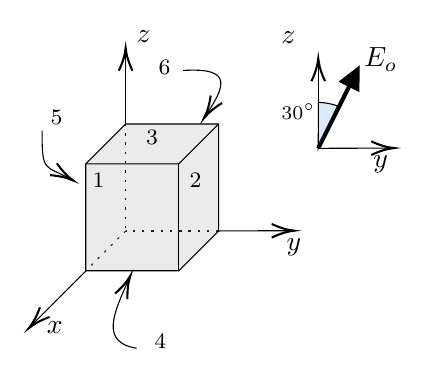
\begin{tikzpicture}[x=0.75pt,y=0.75pt,yscale=-1,xscale=1]
%uncomment if require: \path (0,182); %set diagram left start at 0, and has height of 182

%Straight Lines [id:da9444440815278121] 
\draw  [dash pattern={on 0.84pt off 2.51pt}]  (67.2,109.8) -- (48,129) ;
%Straight Lines [id:da08991584597208946] 
\draw  [dash pattern={on 0.84pt off 2.51pt}]  (112,109.8) -- (67.2,109.8) ;
%Shape: Cube [id:dp7165941380397529] 
\draw  [fill={rgb, 255:red, 155; green, 155; blue, 155 }  ,fill opacity=0.2 ] (48,77.45) -- (67.2,58.25) -- (112,58.25) -- (112,109.8) -- (92.8,129) -- (48,129) -- cycle ; \draw   (112,58.25) -- (92.8,77.45) -- (48,77.45) ; \draw   (92.8,77.45) -- (92.8,129) ;
%Straight Lines [id:da8844067166176446] 
\draw  [dash pattern={on 0.84pt off 2.51pt}]  (67.2,58.25) -- (67.2,109.8) ;
%Straight Lines [id:da20318238488315155] 
\draw    (48.17,129) -- (21.91,155.25) ;
\draw [shift={(20.5,156.67)}, rotate = 315] [color={rgb, 255:red, 0; green, 0; blue, 0 }  ][line width=0.75]    (10.93,-3.29) .. controls (6.95,-1.4) and (3.31,-0.3) .. (0,0) .. controls (3.31,0.3) and (6.95,1.4) .. (10.93,3.29)   ;
%Straight Lines [id:da381549205527151] 
\draw    (112,109.8) -- (146.5,109.67) ;
\draw [shift={(148.5,109.67)}, rotate = 179.79] [color={rgb, 255:red, 0; green, 0; blue, 0 }  ][line width=0.75]    (10.93,-3.29) .. controls (6.95,-1.4) and (3.31,-0.3) .. (0,0) .. controls (3.31,0.3) and (6.95,1.4) .. (10.93,3.29)   ;
%Straight Lines [id:da7722721770942105] 
\draw    (67.2,58.25) -- (67.2,23.67) ;
\draw [shift={(67.2,21.67)}, rotate = 90] [color={rgb, 255:red, 0; green, 0; blue, 0 }  ][line width=0.75]    (10.93,-3.29) .. controls (6.95,-1.4) and (3.31,-0.3) .. (0,0) .. controls (3.31,0.3) and (6.95,1.4) .. (10.93,3.29)   ;
%Straight Lines [id:da5631211047119826] 
\draw [line width=1.5]    (160,70) -- (178.21,33.58) ;
\draw [shift={(180,30)}, rotate = 116.57] [fill={rgb, 255:red, 0; green, 0; blue, 0 }  ][line width=0.08]  [draw opacity=0] (11.61,-5.58) -- (0,0) -- (11.61,5.58) -- cycle    ;
%Straight Lines [id:da8365830796273075] 
\draw    (160,70) -- (194.5,69.87) ;
\draw [shift={(196.5,69.87)}, rotate = 179.79] [color={rgb, 255:red, 0; green, 0; blue, 0 }  ][line width=0.75]    (10.93,-3.29) .. controls (6.95,-1.4) and (3.31,-0.3) .. (0,0) .. controls (3.31,0.3) and (6.95,1.4) .. (10.93,3.29)   ;
%Straight Lines [id:da723347067453898] 
\draw    (160,70) -- (160,28.71) ;
\draw [shift={(160,26.71)}, rotate = 90] [color={rgb, 255:red, 0; green, 0; blue, 0 }  ][line width=0.75]    (10.93,-3.29) .. controls (6.95,-1.4) and (3.31,-0.3) .. (0,0) .. controls (3.31,0.3) and (6.95,1.4) .. (10.93,3.29)   ;
%Curve Lines [id:da5238293302801402] 
\draw    (72.5,166.32) .. controls (55.04,163.41) and (61.1,150.15) .. (68.78,132.93) ;
\draw [shift={(69.5,131.32)}, rotate = 113.96] [color={rgb, 255:red, 0; green, 0; blue, 0 }  ][line width=0.75]    (10.93,-3.29) .. controls (6.95,-1.4) and (3.31,-0.3) .. (0,0) .. controls (3.31,0.3) and (6.95,1.4) .. (10.93,3.29)   ;
%Curve Lines [id:da09178764187978072] 
\draw    (26.93,61.49) .. controls (26.93,81.65) and (27.85,77.85) .. (40.31,84.59) ;
\draw [shift={(41.93,85.49)}, rotate = 209.74] [color={rgb, 255:red, 0; green, 0; blue, 0 }  ][line width=0.75]    (10.93,-3.29) .. controls (6.95,-1.4) and (3.31,-0.3) .. (0,0) .. controls (3.31,0.3) and (6.95,1.4) .. (10.93,3.29)   ;
%Curve Lines [id:da7842102460481515] 
\draw    (94.93,32.49) .. controls (119.89,30.85) and (114.44,40.92) .. (106,53.86) ;
\draw [shift={(104.93,55.49)}, rotate = 303.27] [color={rgb, 255:red, 0; green, 0; blue, 0 }  ][line width=0.75]    (10.93,-3.29) .. controls (6.95,-1.4) and (3.31,-0.3) .. (0,0) .. controls (3.31,0.3) and (6.95,1.4) .. (10.93,3.29)   ;
%Shape: Pie [id:dp592809949302014] 
\draw  [fill={rgb, 255:red, 74; green, 144; blue, 226 }  ,fill opacity=0.2 ] (160.07,47.86) .. controls (160.42,47.87) and (160.78,47.88) .. (161.14,47.9) .. controls (164.05,48.05) and (166.82,48.65) .. (169.36,49.62) -- (160,70) -- cycle ;

% Text Node
\draw (50,80.85) node [anchor=north west][inner sep=0.75pt]  [font=\footnotesize]  {$1$};
% Text Node
\draw (96.8,80.85) node [anchor=north west][inner sep=0.75pt]  [font=\footnotesize]  {$2$};
% Text Node
\draw (75.87,59.77) node [anchor=north west][inner sep=0.75pt]  [font=\footnotesize,rotate=-0.7]  {$3$};
% Text Node
\draw (28,152.4) node [anchor=north west][inner sep=0.75pt]    {$x$};
% Text Node
\draw (143.5,112.07) node [anchor=north west][inner sep=0.75pt]    {$y$};
% Text Node
\draw (71.25,12.13) node [anchor=north west][inner sep=0.75pt]    {$z$};
% Text Node
\draw (141,47.4) node [anchor=north west][inner sep=0.75pt]  [font=\scriptsize]  {$30^{\circ }$};
% Text Node
\draw (185.25,72.4) node [anchor=north west][inner sep=0.75pt]    {$y$};
% Text Node
\draw (141,12.47) node [anchor=north west][inner sep=0.75pt]    {$z$};
% Text Node
\draw (181,20.4) node [anchor=north west][inner sep=0.75pt]    {$E_{o}$};
% Text Node
\draw (79.87,158.42) node [anchor=north west][inner sep=0.75pt]  [font=\footnotesize,rotate=-0.7]  {$4$};
% Text Node
\draw (29.87,50.42) node [anchor=north west][inner sep=0.75pt]  [font=\footnotesize,rotate=-0.7]  {$5$};
% Text Node
\draw (81.87,26.42) node [anchor=north west][inner sep=0.75pt]  [font=\footnotesize,rotate=-0.7]  {$6$};


\end{tikzpicture}


Find the flux through the six labeled faces of the cube with side length $a$ when the electric field is as shown in the diagram. Provide diagrams to justify your equations.

\ifsolutions
\textbf{Solution}

The electric field is parallel to sides 1 and 6, so $\Phi_E^1=\Phi_E^6=0$.

\emph{Method I}



\tikzset{every picture/.style={line width=0.75pt}} %set default line width to 0.75pt        

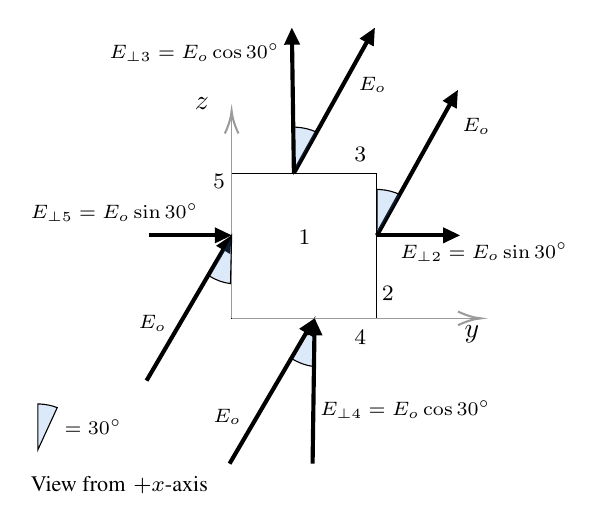
\begin{tikzpicture}[x=0.75pt,y=0.75pt,yscale=-1,xscale=1]
%uncomment if require: \path (0,231); %set diagram left start at 0, and has height of 231

%Shape: Pie [id:dp8757544809507802] 
\draw  [fill={rgb, 255:red, 74; green, 144; blue, 226 }  ,fill opacity=0.2 ] (138.36,163.18) .. controls (134.79,162.72) and (131.22,161.44) .. (127.97,159.37) -- (139,140) -- cycle ;
%Shape: Square [id:dp39107566339579325] 
\draw   (99,70) -- (169,70) -- (169,140) -- (99,140) -- cycle ;
%Straight Lines [id:da8710126107727538] 
\draw [line width=1.5]    (169,100) -- (206.05,33.49) ;
\draw [shift={(208,30)}, rotate = 119.12] [fill={rgb, 255:red, 0; green, 0; blue, 0 }  ][line width=0.08]  [draw opacity=0] (8.13,-3.9) -- (0,0) -- (8.13,3.9) -- cycle    ;
%Straight Lines [id:da036553228152047534] 
\draw [color={rgb, 255:red, 155; green, 155; blue, 155 }  ,draw opacity=1 ]   (99,140) -- (217,140) ;
\draw [shift={(219,140)}, rotate = 180] [color={rgb, 255:red, 155; green, 155; blue, 155 }  ,draw opacity=1 ][line width=0.75]    (10.93,-3.29) .. controls (6.95,-1.4) and (3.31,-0.3) .. (0,0) .. controls (3.31,0.3) and (6.95,1.4) .. (10.93,3.29)   ;
%Straight Lines [id:da09644851790211528] 
\draw [color={rgb, 255:red, 155; green, 155; blue, 155 }  ,draw opacity=1 ]   (99,140) -- (99,42) ;
\draw [shift={(99,40)}, rotate = 90] [color={rgb, 255:red, 155; green, 155; blue, 155 }  ,draw opacity=1 ][line width=0.75]    (10.93,-3.29) .. controls (6.95,-1.4) and (3.31,-0.3) .. (0,0) .. controls (3.31,0.3) and (6.95,1.4) .. (10.93,3.29)   ;
%Straight Lines [id:da13412680651071018] 
\draw [line width=1.5]    (98,210) -- (136.98,143.45) ;
\draw [shift={(139,140)}, rotate = 120.36] [fill={rgb, 255:red, 0; green, 0; blue, 0 }  ][line width=0.08]  [draw opacity=0] (8.13,-3.9) -- (0,0) -- (8.13,3.9) -- cycle    ;
%Straight Lines [id:da953112457460144] 
\draw [line width=1.5]    (129,70) -- (166.05,3.49) ;
\draw [shift={(168,0)}, rotate = 119.12] [fill={rgb, 255:red, 0; green, 0; blue, 0 }  ][line width=0.08]  [draw opacity=0] (8.13,-3.9) -- (0,0) -- (8.13,3.9) -- cycle    ;
%Straight Lines [id:da5946417197466725] 
\draw [line width=1.5]    (58,170) -- (96.98,103.45) ;
\draw [shift={(99,100)}, rotate = 120.36] [fill={rgb, 255:red, 0; green, 0; blue, 0 }  ][line width=0.08]  [draw opacity=0] (8.13,-3.9) -- (0,0) -- (8.13,3.9) -- cycle    ;
%Shape: Pie [id:dp9789969405881314] 
\draw  [fill={rgb, 255:red, 74; green, 144; blue, 226 }  ,fill opacity=0.2 ] (169.07,77.86) .. controls (169.42,77.87) and (169.78,77.88) .. (170.14,77.9) .. controls (173.8,78.09) and (177.23,78.99) .. (180.28,80.45) -- (169,100) -- cycle ;
%Shape: Pie [id:dp19077257181142548] 
\draw  [fill={rgb, 255:red, 74; green, 144; blue, 226 }  ,fill opacity=0.2 ] (129.07,47.86) .. controls (129.42,47.87) and (129.78,47.88) .. (130.14,47.9) .. controls (133.63,48.08) and (136.91,48.91) .. (139.85,50.25) -- (129,70) -- cycle ;
%Shape: Pie [id:dp05387708894606025] 
\draw  [fill={rgb, 255:red, 74; green, 144; blue, 226 }  ,fill opacity=0.2 ] (98.45,123.27) .. controls (94.93,122.83) and (91.42,121.59) .. (88.22,119.58) -- (99,100) -- cycle ;
%Straight Lines [id:da6287683983872696] 
\draw [line width=1.5]    (129,70) -- (128.06,4) ;
\draw [shift={(128,0)}, rotate = 89.18] [fill={rgb, 255:red, 0; green, 0; blue, 0 }  ][line width=0.08]  [draw opacity=0] (8.13,-3.9) -- (0,0) -- (8.13,3.9) -- cycle    ;
%Straight Lines [id:da34533476333963553] 
\draw [line width=1.5]    (169,100) -- (205,100) ;
\draw [shift={(209,100)}, rotate = 180] [fill={rgb, 255:red, 0; green, 0; blue, 0 }  ][line width=0.08]  [draw opacity=0] (8.13,-3.9) -- (0,0) -- (8.13,3.9) -- cycle    ;
%Straight Lines [id:da2544195324607299] 
\draw [line width=1.5]    (138,210) -- (138.94,144) ;
\draw [shift={(139,140)}, rotate = 90.82] [fill={rgb, 255:red, 0; green, 0; blue, 0 }  ][line width=0.08]  [draw opacity=0] (8.13,-3.9) -- (0,0) -- (8.13,3.9) -- cycle    ;
%Straight Lines [id:da3977375610635705] 
\draw [line width=1.5]    (59,100) -- (95,100) ;
\draw [shift={(99,100)}, rotate = 180] [fill={rgb, 255:red, 0; green, 0; blue, 0 }  ][line width=0.08]  [draw opacity=0] (8.13,-3.9) -- (0,0) -- (8.13,3.9) -- cycle    ;
%Shape: Pie [id:dp09036304979526855] 
\draw  [fill={rgb, 255:red, 74; green, 144; blue, 226 }  ,fill opacity=0.2 ] (5.68,181.23) .. controls (6.04,181.24) and (6.4,181.25) .. (6.76,181.27) .. controls (9.67,181.42) and (12.44,182.02) .. (14.98,182.99) -- (5.62,203.37) -- cycle ;

% Text Node
\draw (1,215) node [anchor=north west][inner sep=0.75pt]  [font=\footnotesize] [align=left] {{\fontfamily{ptm}\selectfont View from} $\displaystyle +x${\fontfamily{ptm}\selectfont -axis}};
% Text Node
\draw (130,96.4) node [anchor=north west][inner sep=0.75pt]  [font=\footnotesize]  {$1$};
% Text Node
\draw (88.97,69.24) node [anchor=north west][inner sep=0.75pt]  [font=\footnotesize,rotate=-0.7]  {$5$};
% Text Node
\draw (156.97,144.41) node [anchor=north west][inner sep=0.75pt]  [font=\footnotesize,rotate=-0.7]  {$4$};
% Text Node
\draw (170.17,123.24) node [anchor=north west][inner sep=0.75pt]  [font=\footnotesize,rotate=-0.7]  {$2$};
% Text Node
\draw (210,142.4) node [anchor=north west][inner sep=0.75pt]    {$y$};
% Text Node
\draw (80,32.4) node [anchor=north west][inner sep=0.75pt]    {$z$};
% Text Node
\draw (159,22.4) node [anchor=north west][inner sep=0.75pt]  [font=\scriptsize]  {$E_{o}$};
% Text Node
\draw (17.29,187.4) node [anchor=north west][inner sep=0.75pt]  [font=\scriptsize]  {$=30^{\circ }$};
% Text Node
\draw (39,6.4) node [anchor=north west][inner sep=0.75pt]  [font=\scriptsize]  {$E_{\perp 3} =E_{o}\cos 30^{\circ }$};
% Text Node
\draw (179,102.4) node [anchor=north west][inner sep=0.75pt]  [font=\scriptsize]  {$E_{\perp 2} =E_{o}\sin 30^{\circ }$};
% Text Node
\draw (140.5,178.4) node [anchor=north west][inner sep=0.75pt]  [font=\scriptsize]  {$E_{\perp 4} =E_{o}\cos 30^{\circ }$};
% Text Node
\draw (1,83.4) node [anchor=north west][inner sep=0.75pt]  [font=\scriptsize]  {$E_{\perp 5} =E_{o}\sin 30^{\circ }$};
% Text Node
\draw (209,42.4) node [anchor=north west][inner sep=0.75pt]  [font=\scriptsize]  {$E_{o}$};
% Text Node
\draw (89,182.4) node [anchor=north west][inner sep=0.75pt]  [font=\scriptsize]  {$E_{o}$};
% Text Node
\draw (53,137.4) node [anchor=north west][inner sep=0.75pt]  [font=\scriptsize]  {$E_{o}$};
% Text Node
\draw (156.97,56.41) node [anchor=north west][inner sep=0.75pt]  [font=\footnotesize,rotate=-0.7]  {$3$};


\end{tikzpicture}


$\Phi_E^2=E_oA\cos 60^\circ$, $\Phi_E^3=E_oA\cos 30^\circ$, $\Phi_E^4=E_oA\cos 150^\circ$, $\Phi_E^5=E_oA\cos 120^\circ$

\emph{Method II}

When using this method, it is necessary to draw a diagram to ensure the calculations are correct. The following shows the cube viewed from a point on the $+x$-axis.



\tikzset{every picture/.style={line width=0.75pt}} %set default line width to 0.75pt        

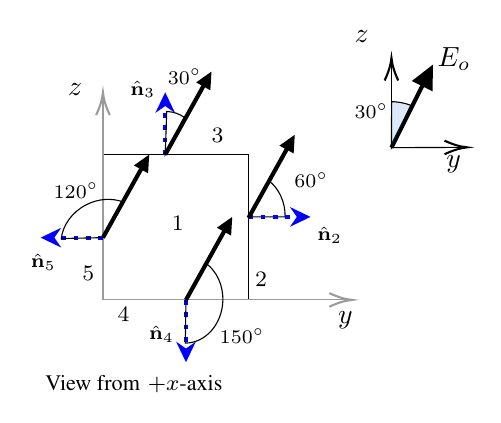
\begin{tikzpicture}[x=0.75pt,y=0.75pt,yscale=-1,xscale=1]
%uncomment if require: \path (0,195); %set diagram left start at 0, and has height of 195

%Shape: Pie [id:dp2468846606935049] 
\draw   (119.83,82.49) .. controls (124.73,86.21) and (127.88,92.7) .. (127.77,100) -- (110,100) -- cycle ;
%Shape: Square [id:dp9965949022820766] 
\draw   (40,70) -- (110,70) -- (110,140) -- (40,140) -- cycle ;
%Straight Lines [id:da9610659135997317] 
\draw [color={rgb, 255:red, 155; green, 155; blue, 155 }  ,draw opacity=1 ]   (40,140) -- (158,140) ;
\draw [shift={(160,140)}, rotate = 180] [color={rgb, 255:red, 155; green, 155; blue, 155 }  ,draw opacity=1 ][line width=0.75]    (10.93,-3.29) .. controls (6.95,-1.4) and (3.31,-0.3) .. (0,0) .. controls (3.31,0.3) and (6.95,1.4) .. (10.93,3.29)   ;
%Straight Lines [id:da413616583119619] 
\draw [color={rgb, 255:red, 155; green, 155; blue, 155 }  ,draw opacity=1 ]   (40,140) -- (40,42) ;
\draw [shift={(40,40)}, rotate = 90] [color={rgb, 255:red, 155; green, 155; blue, 155 }  ,draw opacity=1 ][line width=0.75]    (10.93,-3.29) .. controls (6.95,-1.4) and (3.31,-0.3) .. (0,0) .. controls (3.31,0.3) and (6.95,1.4) .. (10.93,3.29)   ;
%Straight Lines [id:da5430924989686858] 
\draw [line width=1.5]    (40,110) -- (60.34,73.49) ;
\draw [shift={(62.29,70)}, rotate = 119.12] [fill={rgb, 255:red, 0; green, 0; blue, 0 }  ][line width=0.08]  [draw opacity=0] (8.13,-3.9) -- (0,0) -- (8.13,3.9) -- cycle    ;
%Straight Lines [id:da2834934790038013] 
\draw [color={rgb, 255:red, 0; green, 0; blue, 255 }  ,draw opacity=1 ][line width=1.5]  [dash pattern={on 1.69pt off 2.76pt}]  (70,70) -- (70,44) ;
\draw [shift={(70,40)}, rotate = 90] [fill={rgb, 255:red, 0; green, 0; blue, 255 }  ,fill opacity=1 ][line width=0.08]  [draw opacity=0] (9.91,-4.76) -- (0,0) -- (9.91,4.76) -- (6.58,0) -- cycle    ;
%Straight Lines [id:da446424567059891] 
\draw [color={rgb, 255:red, 0; green, 0; blue, 255 }  ,draw opacity=1 ][line width=1.5]  [dash pattern={on 1.69pt off 2.76pt}]  (110,100) -- (136,100) ;
\draw [shift={(140,100)}, rotate = 180] [fill={rgb, 255:red, 0; green, 0; blue, 255 }  ,fill opacity=1 ][line width=0.08]  [draw opacity=0] (9.91,-4.76) -- (0,0) -- (9.91,4.76) -- (6.58,0) -- cycle    ;
%Straight Lines [id:da8656617287924357] 
\draw [color={rgb, 255:red, 0; green, 0; blue, 255 }  ,draw opacity=1 ][line width=1.5]  [dash pattern={on 1.69pt off 2.76pt}]  (80,140) -- (80,166) ;
\draw [shift={(80,170)}, rotate = 270] [fill={rgb, 255:red, 0; green, 0; blue, 255 }  ,fill opacity=1 ][line width=0.08]  [draw opacity=0] (9.91,-4.76) -- (0,0) -- (9.91,4.76) -- (6.58,0) -- cycle    ;
%Straight Lines [id:da677353502578153] 
\draw [color={rgb, 255:red, 0; green, 0; blue, 255 }  ,draw opacity=1 ][line width=1.5]  [dash pattern={on 1.69pt off 2.76pt}]  (40,110) -- (14,110) ;
\draw [shift={(10,110)}, rotate = 360] [fill={rgb, 255:red, 0; green, 0; blue, 255 }  ,fill opacity=1 ][line width=0.08]  [draw opacity=0] (9.91,-4.76) -- (0,0) -- (9.91,4.76) -- (6.58,0) -- cycle    ;
%Shape: Pie [id:dp27262797448521736] 
\draw   (19.93,110.42) .. controls (20.67,104.07) and (24.97,97.81) .. (31.78,94.25) .. controls (37.75,91.13) and (44.33,90.79) .. (49.66,92.79) -- (40,110) -- cycle ;
%Straight Lines [id:da5518439290611417] 
\draw [line width=1.5]    (70,70) -- (90.34,33.49) ;
\draw [shift={(92.29,30)}, rotate = 119.12] [fill={rgb, 255:red, 0; green, 0; blue, 0 }  ][line width=0.08]  [draw opacity=0] (8.13,-3.9) -- (0,0) -- (8.13,3.9) -- cycle    ;
%Straight Lines [id:da7651575856988075] 
\draw [line width=1.5]    (80,140) -- (100.34,103.49) ;
\draw [shift={(102.29,100)}, rotate = 119.12] [fill={rgb, 255:red, 0; green, 0; blue, 0 }  ][line width=0.08]  [draw opacity=0] (8.13,-3.9) -- (0,0) -- (8.13,3.9) -- cycle    ;
%Straight Lines [id:da6060732405226195] 
\draw [line width=1.5]    (110.14,100.45) -- (130.48,63.94) ;
\draw [shift={(132.42,60.45)}, rotate = 119.12] [fill={rgb, 255:red, 0; green, 0; blue, 0 }  ][line width=0.08]  [draw opacity=0] (8.13,-3.9) -- (0,0) -- (8.13,3.9) -- cycle    ;
%Shape: Pie [id:dp06764308064863234] 
\draw   (89.83,122.49) .. controls (94.93,126.36) and (98.14,133.25) .. (97.74,140.92) .. controls (97.16,152.09) and (89.15,160.81) .. (79.68,160.79) -- (80,140) -- cycle ;
%Shape: Pie [id:dp24177309478182996] 
\draw   (70.73,49.22) .. controls (70.84,49.22) and (70.96,49.23) .. (71.07,49.23) .. controls (74.04,49.39) and (76.79,50.38) .. (79.17,52.01) -- (70,70) -- cycle ;
%Straight Lines [id:da7405681093806644] 
\draw [line width=1.5]    (179,66.63) -- (197.21,30.21) ;
\draw [shift={(199,26.63)}, rotate = 116.57] [fill={rgb, 255:red, 0; green, 0; blue, 0 }  ][line width=0.08]  [draw opacity=0] (11.61,-5.58) -- (0,0) -- (11.61,5.58) -- cycle    ;
%Straight Lines [id:da977958020830987] 
\draw    (179,66.63) -- (213.5,66.51) ;
\draw [shift={(215.5,66.5)}, rotate = 179.79] [color={rgb, 255:red, 0; green, 0; blue, 0 }  ][line width=0.75]    (10.93,-3.29) .. controls (6.95,-1.4) and (3.31,-0.3) .. (0,0) .. controls (3.31,0.3) and (6.95,1.4) .. (10.93,3.29)   ;
%Straight Lines [id:da8951841159219021] 
\draw    (179,66.63) -- (179,25.34) ;
\draw [shift={(179,23.34)}, rotate = 90] [color={rgb, 255:red, 0; green, 0; blue, 0 }  ][line width=0.75]    (10.93,-3.29) .. controls (6.95,-1.4) and (3.31,-0.3) .. (0,0) .. controls (3.31,0.3) and (6.95,1.4) .. (10.93,3.29)   ;
%Shape: Pie [id:dp37791603794659623] 
\draw  [fill={rgb, 255:red, 74; green, 144; blue, 226 }  ,fill opacity=0.2 ] (179.07,44.49) .. controls (179.42,44.5) and (179.78,44.51) .. (180.14,44.53) .. controls (183.05,44.68) and (185.82,45.28) .. (188.36,46.26) -- (179,66.63) -- cycle ;

% Text Node
\draw (11,175) node [anchor=north west][inner sep=0.75pt]  [font=\footnotesize] [align=left] {{\fontfamily{ptm}\selectfont View from} $\displaystyle +x${\fontfamily{ptm}\selectfont -axis}};
% Text Node
\draw (72,98.4) node [anchor=north west][inner sep=0.75pt]  [font=\footnotesize]  {$1$};
% Text Node
\draw (28.97,122.41) node [anchor=north west][inner sep=0.75pt]  [font=\footnotesize,rotate=-0.7]  {$5$};
% Text Node
\draw (45.96,142.42) node [anchor=north west][inner sep=0.75pt]  [font=\footnotesize,rotate=-0.7]  {$4$};
% Text Node
\draw (112.17,125.24) node [anchor=north west][inner sep=0.75pt]  [font=\footnotesize,rotate=-0.7]  {$2$};
% Text Node
\draw (152,144.4) node [anchor=north west][inner sep=0.75pt]    {$y$};
% Text Node
\draw (22,34.4) node [anchor=north west][inner sep=0.75pt]    {$z$};
% Text Node
\draw (91.17,56.24) node [anchor=north west][inner sep=0.75pt]  [font=\footnotesize,rotate=-0.7]  {$3$};
% Text Node
\draw (15,82.4) node [anchor=north west][inner sep=0.75pt]  [font=\scriptsize]  {$120^{\circ }$};
% Text Node
\draw (131,77.4) node [anchor=north west][inner sep=0.75pt]  [font=\scriptsize]  {$60^{\circ }$};
% Text Node
\draw (95,152.4) node [anchor=north west][inner sep=0.75pt]  [font=\scriptsize]  {$150^{\circ }$};
% Text Node
\draw (70,27.4) node [anchor=north west][inner sep=0.75pt]  [font=\scriptsize]  {$30^{\circ }$};
% Text Node
\draw (142,103.4) node [anchor=north west][inner sep=0.75pt]  [font=\scriptsize]  {$\hat{\mathbf{n}}_{2}$};
% Text Node
\draw (52,33.4) node [anchor=north west][inner sep=0.75pt]  [font=\scriptsize]  {$\hat{\mathbf{n}}_{3}$};
% Text Node
\draw (4,116.4) node [anchor=north west][inner sep=0.75pt]  [font=\scriptsize]  {$\hat{\mathbf{n}}_{5}$};
% Text Node
\draw (61,151.4) node [anchor=north west][inner sep=0.75pt]  [font=\scriptsize]  {$\hat{\mathbf{n}}_{4}$};
% Text Node
\draw (160,44.03) node [anchor=north west][inner sep=0.75pt]  [font=\scriptsize]  {$30^{\circ }$};
% Text Node
\draw (204.25,69.03) node [anchor=north west][inner sep=0.75pt]    {$y$};
% Text Node
\draw (160,9.1) node [anchor=north west][inner sep=0.75pt]    {$z$};
% Text Node
\draw (200,17.03) node [anchor=north west][inner sep=0.75pt]    {$E_{o}$};


\end{tikzpicture}


The above diagram was used to compute the electric field perpendicular to the side faces.

$\Phi_E^2=E_{\perp 2}A=E_oA\sin 30^\circ$

$\Phi_E^3=E_{\perp 3}A=E_oA\cos 30^\circ$

$\Phi_E^4=E_{\perp 4}A=-E_oA\cos 30^\circ$

$\Phi_E^5=E_{\perp 5}A=-E_oA\sin 30^\circ$

The negative signs in the last two equations were inserted based on the diagram, which shows the electric field points into the volume. These answers are the same as from Method I because $\cos 150^\circ = -\cos 30^\circ$ and $\cos 120^\circ = -\sin 30^\circ$.

\emph{Method III}

This is a problem for which using unit vectors is easier in that an additional diagram is not needed. Compare it to the approach taken in Example 22.2b, pg 728 in the textbook, which is similar to Method I except that an additional diagram was not given (but was likely used to figure out the answer given).

Based on the diagram, $\hat{\mathbf{n}}_1=\ihat$, $\hat{\mathbf{n}}_2=\jhat$, $\hat{\mathbf{n}}_3=\khat$, $\hat{\mathbf{n}}_4=-\khat$
$\hat{\mathbf{n}}_5=-\jhat$, $\hat{\mathbf{n}}_6=-\ihat$

Also, from the diagram, $\mathbf{E}=E_o\sin30^\circ\jhat+E_o\cos30^\circ\khat$.

What remains is to evaluate dot products (you should be able to skip most of the intermediate steps). Using $\mathbf{E}\cdot\mathbf{A}=\mathbf{E}\cdot A\hat{\mathbf{n}}$,

$$\Phi_E^1=\mathbf{E}\cdot \hat{\mathbf{n}}_1A=E_o(\sin 30^\circ\jhat+\cos 30^\circ\khat)\cdot\ihat A = E_oA(\jhat\cdot\ihat\sin 30^\circ+\khat\cdot\ihat\cos 30^\circ)=0$$

$$\Phi_E^2=\mathbf{E}\cdot \hat{\mathbf{n}}_2A=E_o(\sin 30^\circ\jhat+\cos 30^\circ\khat)\cdot\jhat A = E_oA(\jhat\cdot\jhat\sin 30^\circ+\khat\cdot\jhat\cos 30^\circ)=E_oA\sin 30^\circ$$

$$\Phi_E^3=\mathbf{E}\cdot \hat{\mathbf{n}}_3A=E_o(\sin 30^\circ\jhat+\cos 30^\circ\khat)\cdot\khat A = E_oA(\jhat\cdot\khat\sin 30^\circ+\khat\cdot\khat\cos 30^\circ)=E_oA\cos 30^\circ$$

$$\Phi_E^4=\mathbf{E}\cdot \hat{\mathbf{n}}_4A=E_o(\sin 30^\circ\jhat+\cos 30^\circ\khat)\cdot(-\khat A) = -E_oA(\jhat\cdot\khat\sin 30^\circ+\khat\cdot\khat\cos 30^\circ)=-E_oA\cos 30^\circ$$

$$\Phi_E^5=\mathbf{E}\cdot \hat{\mathbf{n}}_5A=E_o(\sin 30^\circ\jhat+\cos 30^\circ\khat)\cdot(-\jhat A) = -E_oA(\jhat\cdot\jhat\sin 30^\circ+\khat\cdot\jhat\cos 30^\circ)=-E_oA\sin 30^\circ$$

$$\Phi_E^6=\mathbf{E}\cdot \hat{\mathbf{n}}_6A=E_o(\sin 30^\circ\jhat+\cos 30^\circ\khat)\cdot(-\ihat A) =  -E_oA(\jhat\cdot\ihat\sin 30^\circ+\khat\cdot\ihat\cos 30^\circ)=0$$

Checks: The flux is positive for faces 2 and 3. This is consistent with the diagram because if electric field lines were drawn, they would emerge from the volume out of these faces. The flux is negative for faces 4 and 5. This is consistent with the diagram because if electric field lines were drawn, they would enter the volume.
\fi

\end{document}